\section{O Sistema de Limpeza}
\subsection{Os Filtros}
A filtragem irá garantir que a piscina estará limpa após o uso do \textit{Clean Pool Robot}. O filtro será fundamental, pois ele será responsável pela remoção das partículas de sujeira que ficam decantadas no fundo da piscina. Primeiro a água será sugada para dentro do aparelho que passará por um depósito onde será feita a filtragem. Em seguida, a água filtrada retorna para piscina. Será realizado um sistema de dupla filtragem com dois tipos de elementos filtrantes: um de malha de alumínio, elemento secundário, para evitar que folhas e objetos de maior tamanho entrem no filtro principal que será responsável por filtrar o particulado e detritos da água.

Será usada uma malha de alumínio para a realização de uma pré-filtragem, que impedirá que folhas, plásticos, cabelos, e outros materiais maiores entupam o filtro principal responsável por retirar impurezas menores da água. Essa malha é o que chamou-se de filtro secundário. O filtro principal será um elemento filtrante na forma cilíndrica comumente utilizado na filtragem de caixas d’águas. As imagens dos filtros a serem utilizados e as especificações técnicas do elemento filtrante principal constam a seguir. Juntamente com o sistema de filtragem existe o que se chamou de “caixa de sujeira”, nela as pedras, folhas, galhos e outros objetos que poderam entupir ou diminuir a vazão de filtragem serão armazenadas. Essa caixa deverá ser limpa sempre que o robô for retirado da água.
\begin{description}
\item[Malha de Alumínio:] A malha de alumínio é um material durável, altamente resistente a água, não precisa de manutenção e nem de troca. Em caso de avaria na grade a substituição é simples e barata. A grade será localizada na entrada da caixa filtradora, no duto de acesso na base do robô, conforme Figura \ref{fig:mesh-aluminium}.
\par
  \begin{figure}[h]
    \centering
    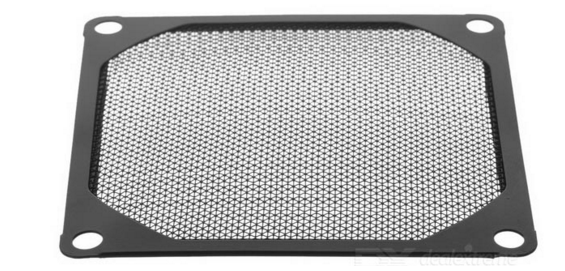
\includegraphics[width=0.8\textwidth]{figures/mesh-aluminium.png}
    \caption{Modelo de malha de alumínio utilizada como filtro secundário.}
    \label{fig:mesh-aluminium}
  \end{figure}
  \FloatBarrier
\par
\item[Elemento Filtrante:] as seguintes características são requeridas.

\begin{itemize}
\item Temperatura de operação: 5ºC mín. a 50ºC máx.
\item Vazão: 4.200 litros/hora
\item Grau de filtração: 50 micra (um grão de areia tem entre 200 a 500 micra)
\item Peso bruto: 448g
\item Peso líquido: 337g
\end{itemize}
Para se garantir a qualidade da água filtrada é indicado pelo fabricante a substituição dos elementos filtrantes \textit{Poly Flow} a cada 6 meses ou quando for observada a redução do fluxo da água. O elemento filtrante é descartável, não necessita retrolavagem. A manutenção periódica do elemento é aconselhável. Para isso, utilize apenas água e uma escova macia.

Dimensões: Altura: 254mm; Diâmetro externo: 116mm; Diâmetro interno: 26mm.
\par
  \begin{figure}[h]
    \centering
    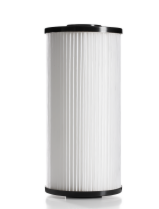
\includegraphics[width=0.2\textwidth]{figures/filter.png}
    \caption{Elemento Filtrante}
    \label{fig:filter}
  \end{figure}
  \FloatBarrier
\par
O elemento filtrante na forma cilíndrica, além de ser o mais encontrado comercialmente, proporcionará ao \cpr uma compactação dos dutos de filtragem e uma melhor organização interna para alocação de seus componentes. O modelo de filtro selecionado da \textit{Poly Flow} e similares é o que mais se encaixa as necessidades de projeto e ao volume de trabalho da bomba a ser utilizada. Esses modelos são comumente utilizados na filtragem de caixas d’águas, piscinas e banheiras.
\end{description}

\subsection{O Dimensionamento dos Filtros}
Os filtros foram dimensionados, ou escolhidos, a partir dos pré-requisitos do projeto, isto é, velocidade, limpeza, área de atuação. Após a análise do que deveria ser filtrado e das possíveis fontes de entupimento do sistema de filtragem, dividiu-se o sistema em 3 áreas: caixa de sujeira; filtro secundário; filtro principal. 

\subsection{Os Rolos de Limpeza}
Das principais sujeitas depositadas no fundo de piscinas pode-se listar: folhas e pequenos gravetos de arvores presentes nos arredores, além do acúmulo de algas, fungos e bactérias no fundo. Como solução para a limpeza destas sujeiras a utilização de peças com superficies mais macias ajudam a desgrudar do fundo as impurezas, independente de qual for o revestimento da piscina, se ele for azulejo, vinil, fibra ou pintura.(7)

Os rolos de limpeza estão localizados na parte frontal e traseira do robô, e  terão duas funções: a principal é auxiliar na remoção das impurezas do fundo da piscina, e a função secundária se dá no auxilio a sustentação do robô.

Para o processo principal, a remoção das pequenas partículas depositadas no fundo da piscina, o rolo irá deslizar sob a superfície, sem que seja produzido muito atrito, para que não altere a velocidade total do robo e não danifique a superfície. Assim, o material do rolo deve ser macio, leve e ao mesmo tempo resistente a água.

Para o processo secundário, de auxílio a sustentaçao do robô os rolos devem ter o seu raio na distância do fundo da piscina até a entrada de sucção, ou seja, a altura das rodas, pois assim o robô ficará nivelado e ao mesmo tempo com apoio na frente, atrás e no centro. Para esse requisito, o atendimento do \textit{design} proposto, os rolos deverão ter, cada um deles, 300 mm de comprimento, 60 mm de diâmetro total e um eixo central com 30 mm de diâmetro, no qual será encaixado os eixos de rotação para os motores.

Definiu-se primeiramente utilizar escovas de formato cilíndrico e de \textit{Nylon}, afim de que á medida que as rodas do robô se movem, as escovas também possam acompanhar o movimento sem maiores problemas. Porém a dificuldade em encontrar fabricantes e modelos em Brasília e devido também ao elevado custo decidiu-se pela fabricação das escovas. Para a fabricação usou-se um tubo 50 mm de pvc e um revestimento de polimero, a fibra de vinil.

A utilização de um polímero possui várias vantagens, tais como: baixa densidade, alta resistência à corrosão, baixo custo de aquisição, coeficiente de atrito baixo e grande flexibilidade. O baixo custo e densidade foram os principais motivos para a realização da troca.
\par
  \begin{figure}[h]
    \centering
    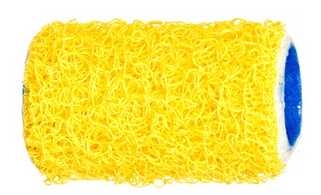
\includegraphics[width=0.5\textwidth]{figures/brush-vinil.png}
    \caption{Rolo de fibra de vinil.}
    \label{fig:brush-vinil}
  \end{figure}
  \FloatBarrier
\par
